\Chapter{Storing plot state of a game world}

\section{Plot events}

Saussure introduced the distinction between language (la langue) and meaning (la parole)\cite{gordon2004langue}.
When thinking about how to represent the plot state of the game world, one should take into account the possible space of expression within it.
%
In Saussure's framework, language (la langue) refers to the overall system of rules, conventions, and structures that govern a particular language, while meaning (la parole) refers to the individual utterances or expressions produced by speakers of that language.
This distinction emphasizes the idea that language is a system that is shared and agreed upon by a community of speakers, and that meaning is not fixed but rather is created through the interaction between the language system and the speaker's intentions and context.
When representing the plot state of a game world, it is important to consider the language used to describe that world and the range of expressions that are possible within that language.
%
In general, plot representation should be able to express a chronological event with some relevance to the story.
A story is a collection of plots.
Each plot may be considered in the scope of multiple narratives.
For the sake of plot representation, the important aspect is in being able to convey the event in an impartial manner without taking into account the narrative within which it can be considered.
As noted by Lindley, the plot state of the game world does not need to be available and presented to the player in its entirety, as is the case for example in games such as SIM City \cite{lindley2005story}.
In general, the player only has access to a given subset of the plot state as they discover each individual plot point separately.
The same can be said about the simulated actors in the game world as limiting their knowledge may increase the realism of the simulation and in turn result in a more immersive experience.

The two most commonly used formalism for representation of plot state in games are situation calculus and event calculus.
The situation calculus is a logical language for representing changes\cite{lin2008situation}.
According to Levesque, in situation calculus "the foundational axioms for situations provide a purely qualitative notion of time whose only temporal concept is sequential action occurrence: an action occurs before or after another within"\cite{levesque1998foundations}.
The event calculus is a formalism for reasoning about action and change \cite{mueller2008event}.
Similarly to the situation calculus, the event calculus uses the concept of actions (called "events") and fluents.
The main difference is that events can be external and happen at specific time points which makes it essential for modelling plot state where a plot event can happen in isolation.
Event calculus was introduced first in 1986 by Kowalski and Sergot \cite{kowalski1986logic}.
It was then simplified in 1992 \cite{kakas1992abductive}.

In general, plot state of a game world can be represented in a plethora of ways, depending on the defined use cases.
Plot state can be associated with the state of knowledge in a given region or with an individual actor.
The first approach is used for spatial modelling where the game world is partitioned into disjoint regions that can be considered to be homogeneus in terms of their reaction to various kinds of plot events.
The second approach is useful for creation of logical models that may be employed to simulate very precise and complex interactions between individual actors.
It is worth mentioning that an actor does not necessarily need to be a representation of a person but may as well be a whole region, a city, a town or even an abstract concept.
Spatial models are well suited for simulating how a given plot even will impact the rest of the game world in terms in terms of information propagation.
Logical models excel in representing complex interactions and simulating how actors relay information about plot events to each other and thus gain knowledge on the state of the plot state in the game world.

\section{Logical models}

A logical model is called an information network.
It consists of a set of actors and information pathways between them.
An actor holds limited knowledge about the game world.
An information pathway is a physical possbility of an actor to exchange information with another actor.
Activation of an information pathway can be thought of as a conversation between the two interconnected actors.
An example of an information network can be seen on figure \ref{fig:logical_model_example}.

\begin{figure}
    \centering
    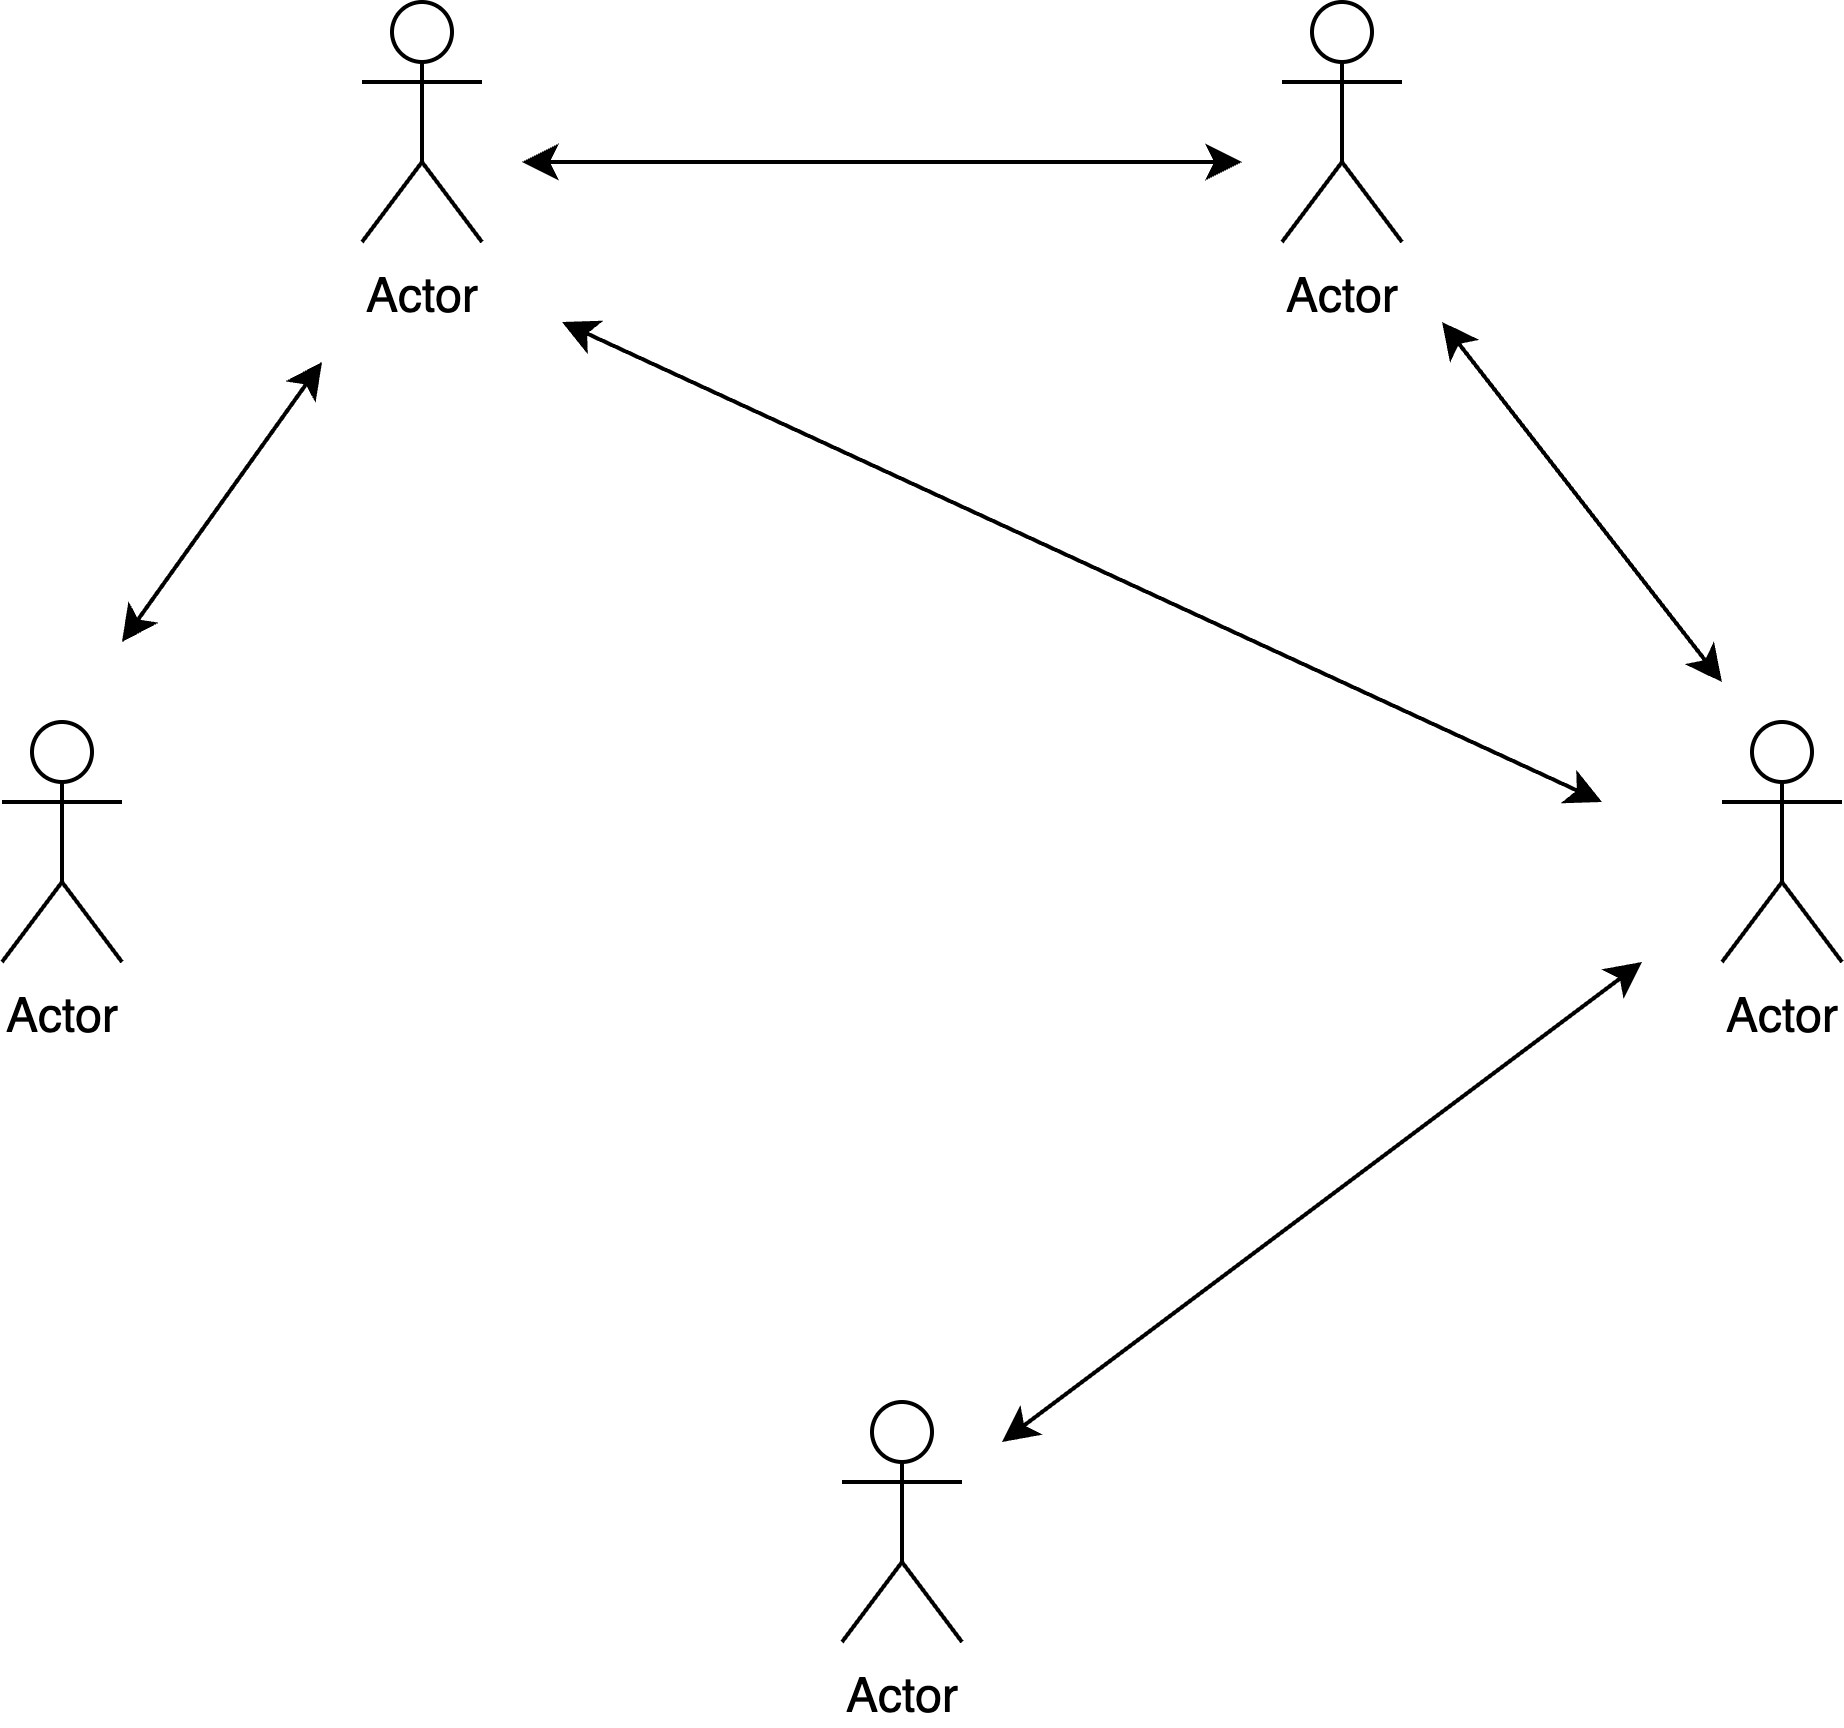
\includegraphics[width=0.6\textwidth]{images/logical_model_example.png}
    \caption{Example of an information network}\label{fig:logical_model_example}
\end{figure}

\section{Spatial models}

WIP

\section{Partitioning of actors to form spatial models}

Spatial models can be constructed by partitioning a logical model after assigning each actor its physical location and calculating bounds of each logical network.
This method requires that actors form disjoint sets of information networks.
Any plot even propagated to each spatial region can be either made immedietely accessible to all members of the embedded logical model or to a specific subset of actors.
Similarly an actor may be designated a gateway out of the logical model into the spatial one and gain the ability to propagate information to other spatial regions.
This way a game world may employ both types of models to essentially store the whole plot state and simulate in detail only the subset of regions that the player is in close proximity to.
This approach makes usage of the logical model a viable solution for large scale open world games.

\section{Difference between knowledge and information}

% What is information?
The most important distinction when building information propagation models is the one that differentiates knowledge from information.
The latter can be propagated while the former cannot.
This is due to the fact that information represents a statement of fact, irrespective of whether it is true or not.
A claim that people with axes are walking down the road towards the forest can be an information.
It should be considered to be fundamentally literal and represent nothing more than the messaging mechanism used to convey it.

% Knowledge
A person has a mind capable of linking events, seeing connections between facts, identifying patterns and inferring new knowledge from received information.
Anyone can easily see that such a group of aforementioned people can represent lumberjacks aiming to chop down the trees.
Note that neither the word lumberjack or the act of chopping down any tree was mentioned before.
This shows the distinction between what is pure information and what can be considered knowledge.
After all, how does one come to the conclusion that axes and trees must mean lumberjacks?
One needs to be aware of the concept of an axe and its function as well as the existence of the trade of forestry to make that connection.

% Propagation
After realizing the meaning of people with axes going towards a forest, one can decide to tell others of this news by formulating a new statement of fact: "Lumberjacks are going to the forest".
A more natural example would be a person telling a friend that someone told them about a group of lumberjacks heading to a forest.
This is an example of information propagation.
It can be illustrated more clearly by assuming the person who heard about the people heading towards the forest had recently seen a pack of wolves in the area.
They might get alarmed and wish to warn the unsuspecting workers.
The information "there are wolves in the forest" has the characteristic of urgency as well as importance.
It is urgent because telling it after the workers get to the forest misses the whole point of warning them.
It is important because it influences their safety.
These two factors lay the foundation for best possible propagation effect.
One would immedietely embark on a trip to warn the lumberjacks of the dangers lurking in the forest and probably mention the situation to anyone they pass by.
This particular situation also has the characteristic of being targeted towards a specific group.

% TODO: Find characteristics of information in literature
% Information characteristics
Information can be urgent, important and have a target group of receiving people.
Urgency determines the temporal aspect of propagation.
Importance influences how much effort one is willing to spend delivering the information.
A target audience limits the list of potential receivers.
An information can be urgent and not important, that would simply mean that it will expire after some limited time but if the effort to deliver it on time is too great, it is possible that it won't be done.
It can be important but not urgent just as well.
In this case it means that it must be delivered but there are no consequences to doing so later rather than sooner.
It is worth noting however that importance also influences the temporal element of information propagation as more important messages are going to be propagated faster.
A target audience can be homogeneus (a group of lumberjacks) or have a variety of different people.
A person doing the propagation can have a list of intended recipents of a message they are carrying.
There can also be people who are subscribers of selected kinds of information.
A mother would like to know if anything happens to her child and as such one can say she subscribes information regarding the health of her children.
In real life there are many more aspects and characteristcs that are deeper and more nuanced that what was described.
No artifical model can represent accurately the intricacies of the human mind, much less a group of minds.

% How information and knowledge interact
Information cannot exist without someone to perceive it and knowledge cannot exist without information.
Whenever there is some entity that is able to receive information and understand it, it can produce knowledge.
Information nececessitates a receiver to exist somewhere in the system that can produce knowledge.
This means that all three must always be present.
Collections of actors able to receive information and process it into knowledge as well as create new information and share it with other actors will be henceforth reffered to as information systems.

% Complexity of information systems
An information system is a set of actors possessing knowledge and wishing to spread it in the form of information.
Because the complexity of real information systems is too great, simplification needs to be made in order to focus on the important aspects of such a system.
We can identify the key elements of any information system:
\begin{itemize}
    \item Actor - a person capable of processing information, holds knowledge and can produce new information
    \item Information - statement originating from any information source, ie. an actor
    \item Information source - any source of information, can be an actor or an inanimate source such as a recording or text
    \item Information pathway - any link between actors through which information can travel, can affect the information causing distortion or impact the propagation
\end{itemize}
Actors may be offered information or they might produce information themselves.
This must always happen through an information pathway.
Inanimate sources of information, ie a written book, may exist within the same system and are considered to be always producing some (usually constant) information.
An actor may react differently when offered different kinds of information or even the same one repeatedly.
To illustrate that one can imagine being interested in buying a new pair of shoes if seeing the advertisment of them for the first time and getting more annoyed each consecutive time the same advertisment is played.
% TODO: Cite the work modelling marketing strategy effectiveness
This behaviour is usually the target of marketing strategy analysis as simply increasing the intensiveness of advertisment broadcast will not increase the demand for the shown product.
Aside from being able to receive information, an actor may decide to share it with other actors.
They might decide to choose a target group or broadcast it to everyone they can reach.
Some actors may seek certain types of information and query for it anytime they can.
In order to do so, actors must possess some knowledge.

% Complexity of knowledge
Knowledge is a set of statements about the world that are consistent (irrespective of truthfulness).
One can claim that the planet is flat while another person might disagree and it is valid to say that both possess knowledge about the shape of the world.
A person can then infer new facts on the basis of what they already know and for instance make a claim that travelling past the edge of the Earth will cause the daring explorer to fall to their demise.
The second person will then receive such information and basing on their opposing set of known statements will reject it and possibly reduce the opinion of the first person, being less likely to believe anything they might then tell them.
It is however impossible to model the interactions between information necessary to infer new information the same way that happens in the human mind, at the very least not in any feasible way.
The complexity of interconnectedness of knowledge and information alike is too great to be represented fully.
One can however make assumptions and put constraints on the type of statements allowed and the knowledge that can be gained and thus create a simplistic representation of an information system.

% Scope - logical vs spatial
There are two main types of information systems that can be used to model information propagation:
% TODO: Add some citation to "podział przestrzeni na abstrakcyjną i fizyczną"
\begin{itemize}
    \item spatial - they model information spread across space, usually partitioned into homogeneus segments or tiles
    \item logical - representing connections between actors without taking into account physical relationships between them
\end{itemize}
The first kind of information system, spatial information systems (SIS) can be used to model large scale events happening across the world.
The most important assumption in these kind of systems is the homogenuity of any given unit of space as defined by the chosen partitioning method.
They assume that information has some kind of physical propagation characteristic that allows it to travel across space.
In these systems an actor needs not to be represented individually but rather can be treated as part of a homogeneus group.
This model might be used to represent how news regarding the death of a ruler might spread from the captial to the most remote villages.
The second type of information systems, logical information systerms (LIS) work on the basis of individual actors and interactions between them.
They are ill suited for large scale modelling as the number of actors to be considered would grow considerably.
Of course, a spatial system can be represented as a logical system if some of the more important regions of the spatial model are chosen and represented as actors in the logical model.

% What does it mean for information to be considered as propagated?
The process of propagating information from one actor to another can be considered in the scope of physical information receival as well as logical aspect of interpretation.
The act of knowledge assimilation is inherently present in the process of actor receiving information from any external source.
% Is it sufficient to transfer information from source to target?
Information can reach its target in a plethora of ways.
In many models
% What happens after information reaches the target?
% What are the sources of information?

% Plot events: 
% Śmierć władcy rozprzestrzeni się od punktu centralnego wzdłuż dróg
% Wybuch wulkanu rozprzetrzeni się od każdego miejsca z którego był widoczny
% Smok będzie widziany na całej jego trasie lotu, uwzględniając czas.
% Epidemia, każdy nowy chory ma większy priorytet

\section{Representation of information}

Modelling propagation of information itself is possible without looking at how it is represented.
The same is not true for modelling knowledge and its interaction with the former.
The ability to express any concept relies on the application of language.
It is precisely that which enables and also limits everything that is able to be conveyed using it.
Natural language is very complicated and full of inconsistencies.
Human brain handles that very well and in fact often is the source of said inconsistencies.
In order to create a model useful in terms of game development, it needs to have a clearly defined way to represent information.
One such option is the application of relational algebra.
To create a language one needs to think about what concepts it should allow expression of.
For example, in the English language a very simple sentence can be assembled: "The apple is red".
This sentences implies several things about the state of the described world.
First and foremost it implies the existence of a specific apple.
Secondly, it implies that apples have the attribute of color and that this particular one is red.
Due to its simple nature, both semantically and syntatically, one could write the following mathematical representation of this sentence:

$$
    \left( apple, is, red \right)
$$

An ordered set of words that in the right context is understood to mean that there exists an apple and that said apple is red.
A reasonable assumption is that by having a sufficiently sophisticated representation, it should be possible to tell whether a given pair of such statements are conflicting.

$$
    \left( apple, is, red \right) \neq \left( apple, is, green \right)
$$

To a human such an equation will seem correct at first glance.
However, as previously mentioned, the word "red" carries an impliciation of the described object possessing the attribute of color.

$$
    \left( apple, is, red \right) \neq \left( apple, is, round \right)
$$

The above statement is false as it tries to compare two distinct attributes, namely shape and color.
In order to make these kinds of statements more explicit, a fourth element is added.

$$
    \left( apple, is, color, red \right)
$$

This way it is possible to represent any arbitrary statement in the form of: "Object $X$ has attribute $Y$ of value $Z$" in the form of:

$$
    \left( X, is, Y, Z \right)
$$

In terms of relational algebra one can think of the word "is" as an operator denoting a binary relation between some object and the value of some attribute.
Because a language should have more than a single type of expressable relation, the mathematical representation should be more generic to accomodate all kinds of binary relations:

$$
    \left( operator, first, second \right)
$$

In the case of the $is$ operator:

$$
    \left( is, object, \left\{ attribute, value \right\} \right)
$$

Following the previous example:

$$
    \left( is, apple, \left\{ color, red \right\} \right)
$$

Then, one can define a function determining whether two statements $S_a$ and $S_b$ are conflicting:

$$
    S_a = \left( is, x_a, \left\{ y_a, z_a \right\} \right)
$$

$$
    S_b = \left( is, x_b, \left\{ y_b, z_b \right\} \right)
$$

$$
    conflict \left( S_a, S_b \right) \iff x_a = x_b \land y_a = y_b \land z_a \neq z_b
$$

% Identity
One important aspect of the natural language is ambiguity of subject's identity.